\subsection{Selección Monogamica Aleatoria}
Es un mecanismo similar a la selección monogámica aleatoria, con la peculiaridad de que una vez que un individuo a sido seleccionado, no se puede volver a seleccionar en esa generación. Este algoritmo garantiza que todos los individuos se reproduzcan, sin embargo, esto podría traer el problema de que prevalezcan individuos no aptos. La Figura \ref{fig: selection_mono} muestra una representación gráfica de este proceso.

\begin{figure}[htbp]
	\centering
	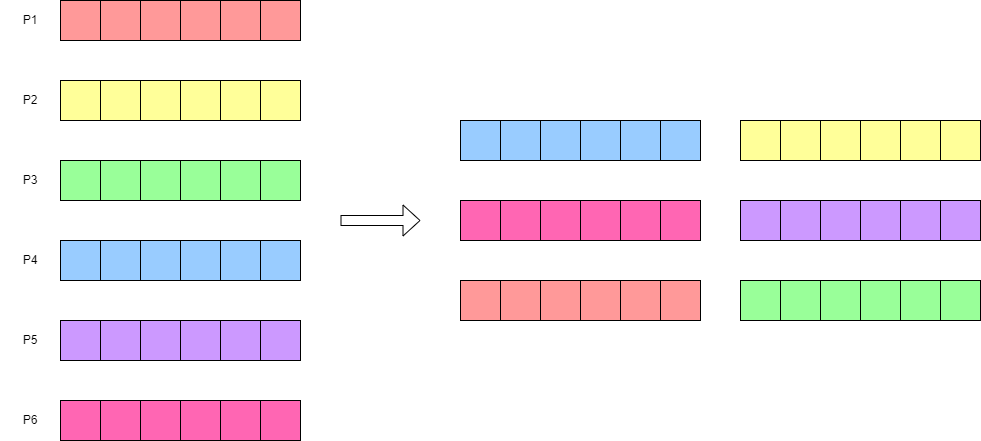
\includegraphics[width=0.8\textwidth]{random_monogamica}
	\caption{Mecanismo de selección monogámica aleatoria.}
	\label{fig: selection_mono}
\end{figure}


\subsection{Partially Mapped Crossover}
El Partially Mapped Crossover (PMx) es una técnica de cruce especialmente diseñada para problemas de optimización combinatoria en los que las soluciones son representaciones de permutaciones de números. El objetivo del PMx es transferir sin ambigüedades segmentos de información entre dos padres, garantizando que los hijos resultantes sean permutaciones válidas.

El algoritmo consta de la siguiente serie de pasos:

\begin{enumerate}
	\item Selección de un Segmento: Se seleccionan aleatoriamente dos puntos de corte en los padres, que definen un segmento.1
	\item Intercambio de Segmentos: Se intercambian los segmentos entre los dos padres para formar la base de los dos hijos.
	\item Reemplazo Fuera del Segmento: Para cada posición fuera del segmento intercambiado:
	\begin{enumerate}
		\item Si el número en la posición correspondiente del otro padre ya está presente en el segmento intercambiado, se busca el número que ocupa esa posición en el segmento original y se sigue rastreando las posiciones hasta encontrar un número que no esté en el segmento intercambiado.
		\item Se reemplaza el número en la posición actual del hijo con el número encontrado en el paso anterior.
	\end{enumerate}
	\item Finalización: Se repite el paso anterior hasta que todos los números fuera del segmento intercambiado en ambos hijos son permutaciones válidas de los números originales.
\end{enumerate}

Este mecanismo se puede representar gráficamente como se muestra en la Figura \ref{fig:PMx}.

\begin{figure}[htbp]
	\centering
	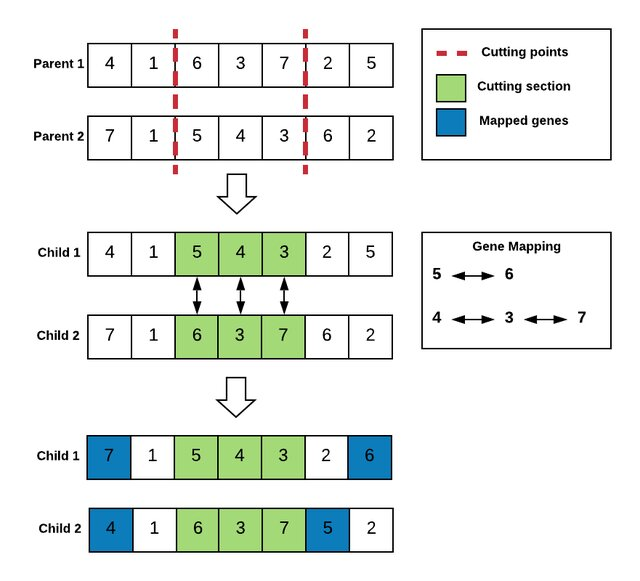
\includegraphics[width=0.7\textwidth]{pmx}
	\caption{Diagrama de funcionamiento de partially mapped crossover.}
	\label{fig:PMx}
\end{figure}


\subsection{Scramble Mutation}
La mutación por mezcla (scramble mutation, en inglés) es un proceso que introduce pequeños cambios aleatorios en los individuos de una población con el objetivo de aumentar la diversidad genética y explorar nuevas soluciones en el espacio de búsqueda. Dicho proceso se caracteriza por los siguientes pasos:

\begin{enumerate}
	\item Selección de un subconjunto de genes: Se elige un subconjunto aleatorio de genes en la representación del individuo. Los genes seleccionados formarán parte del proceso de mutación.
	\item Mezcla de genes: Los genes seleccionados se reordenan de manera aleatoria entre sí. Este reordenamiento aleatorio puede ser realizado de diferentes maneras, como permutando los valores de los genes dentro del subconjunto o cambiando su posición en la secuencia.
\end{enumerate}

Podemos observar una representación gráfica de este mecanismo en la Figura \ref{fig:scrM}.

\begin{figure}[htbp]
	\centering
	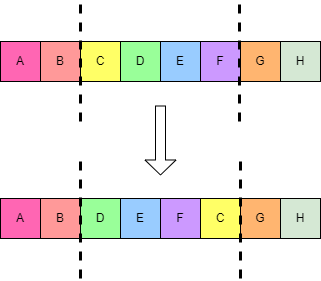
\includegraphics[width=0.4\textwidth]{scramble_mutation}
	\caption{Diagrama de funcionamiento de scramble mutation.}
	\label{fig:scrM}
\end{figure}

\subsection{Búsqueda Tabú}
La búsqueda tabú es una técnica que se utiliza en el contexto de algoritmos genéticos y otros algoritmos de optimización para evitar la convergencia prematura hacia una solución subóptima. Ayuda a diversificar la búsqueda y explorar un espacio de soluciones más amplio. La búsqueda tabú se basa en la idea de mantener un registro de soluciones prohibidas o "tabúes" que no se deben explorar nuevamente durante un cierto período de tiempo. Estas soluciones prohibidas se almacenan en una lista llamada lista tabú.
